\section{The Doob-Gillespie Algorithm in Detail with Examples}\label{sec:algorithm}

%\textbf{Instructional Hours:} 12-18 hours

The Doob-Gillespie algorithm uses the ODE parameters and initial conditions to generate a \textit{stochastic trajectory}\index{trajectory!stochastic}. The word \textit{stochastic} means \textit{random}. Unlike ODE solutions, which system parameters and initial conditions fully determine, a stochastic trajectory is one possible random realization of the system evolution. Concretely, a stochastic trajectory is a sequence of time-state tuples $(t_0, {\tt state}_0), (t_1, {\tt state}_1), (t_2, {\tt state}_2), \ldots$, where $(t_i, {\tt state}_i)$ records the time and system state immediately after the $i^{th}$ state-change event occurs. The algorithm proceeds as follows. Steps 0 and 1 are pre-processing steps: run them once before any simulation begins. Step 2 initializes the simulation bookkeeping. Steps 3 and forward constitute the main loop, which repeats while the clock $t$ remains below the simulation run time $T$.
\begin{enumerate}
\item[\textbf{Step 0.}] (Pre-processing.) Scale\index{rescaling} and/or re-parameterize\index{re-parameterization} the system so that the state variable counts discrete individuals. Perform this step once, before the simulation loop begins.
\item[\textbf{Step 1.}] (Pre-processing.) Identify all the state-change events $\left\{E_i\right\}_i$ and their effects on the state $\left\{\delta_i\right\}_i$.
\item[\textbf{Step 2.}] (Initial bookkeeping.) Set $t = 0$, set the state to the initial conditions, and record the time and state.
\item[\textbf{Step 3.}] Use the current state to compute the rate $\lambda_i$ of each event.
\item[\textbf{Step 4.}] Compute the total rate $\lambda = \sum_i \lambda_i$ and the PMF $p_i = \lambda_i/\lambda$.
\item[\textbf{Step 5.}]   If $\lambda = 0$, terminate. 
\item[\textbf{Step 6.}] Sample $U \sim \text{Uniform}(0,1]$ and compute $\Delta t \sim Exp(\lambda)$ by setting $\Delta t = -\ln(U)/\lambda$.
\item[\textbf{Step 7.}] Sample $W \sim \text{Uniform}(0,1]$, compute the index $j$ of the next event $E_j$ from the PMF $\left\{p_i\right\}_i$ by setting $j = \min\left\{k \middle| \sum_{i \leq k} p_i \geq W\right\}$, and look up the state-change event $\delta_j$.
\item[\textbf{Step 8.}] Update the clock $t \leftarrow t + \Delta t$, the state $\texttt{state} \leftarrow \texttt{state} + \delta_j$, record the new time and state, and, if $t < T$, go back to step 3.
\end{enumerate}

The algorithm calls five subroutines: $\textsf{MakeDeltaStates}$ tabulates the state changes once in Step 1, and the main loop then calls $\textsf{MakeRates}$ to evaluate the event rates, $\textsf{RatesToPmf}$ to form the PMF and total rate, $\textsf{RateToDeltaTime}$ to sample the waiting time, and $\textsf{PmfToEventIndex}$ to select the next event.
Note that computing rates, and looking up the state-change event after sampling an index $j$, both depend on the ODE model.
All else is the same for every ODE model, and we implement it generically. We index the $n$ events from $0$ to $n-1$ throughout, matching the companion \texttt{Python}.

We assemble these subroutines into the full algorithm. Figure~\ref{fig:dg_algorithm} presents it symbolically, the numbered steps above explain it, and each line of the figure shows its step. Figures~\ref{fig:dg_subroutines_a} and~\ref{fig:dg_subroutines_b} collect the pseudocode for the five subroutines it calls. Listing~\ref{lst:dg_algorithm_python_template} gives the \texttt{Python 3.12} implementation, a template that follows the same steps line for line. It diverges from the pseudocode only at Step 5: rather than breaking out of the loop, it returns the trajectory as soon as \RatesToPmf{} yields a total rate of zero.

\begin{figure}[htbp]
\centering
{\footnotesize
\fbox{\procedure{Doob-Gillespie Algorithm $\textsf{DG}(T,\, x_0,\, \theta) \to \textsf{traj}$:}{
\pcind (\delta_j)_{j=1}^{N} \leftarrow \textsf{MakeDeltaStates}(\theta)\,; \pccomment{\text{Step 1}}\\
\pcind t \leftarrow 0 \,;\; x \leftarrow x_0 \,;\; \textsf{traj} \leftarrow [(0,\, x_0)]\,; \pccomment{\text{Step 2}}\\
\pcind \pcwhile t < T \pcdo \\
\pcind\pcind \vec{\lambda} \leftarrow \textsf{MakeRates}(x,\, \theta)\,; \pccomment{\text{Step 3}} \\
\pcind\pcind (\vec{p},\, \lambda) \leftarrow \textsf{RatesToPmf}(\vec{\lambda})\,; \pccomment{\text{Step 4}}\\
\pcind\pcind\pcif \lambda = 0 \pcthen \textbf{break}\,; \pccomment{\text{Step 5}} \\
\pcind\pcind \Delta t \leftarrow \textsf{RateToDeltaTime}(\lambda)\,; \pccomment{\text{Step 6}} \\
\pcind\pcind j \leftarrow \textsf{PmfToEventIndex}(\vec{p})\,; \pccomment{\text{Step 7}} \\
\pcind\pcind t \leftarrow t + \Delta t \,;\; x \leftarrow x + \delta_j \,; \pccomment{\text{Step 8}} \\
\pcind\pcind \textsf{traj} \leftarrow \textsf{append}\left(\textsf{traj}, [(t,\, x)]\right)\,; \\
\pcind\pcendwhile\\
\pcind \pcreturn \textsf{traj}
}}}
\caption{Doob-Gillespie algorithm, Steps 1 to 8. Here $T$ is the simulation run time, $x_0$ is the initial state, $\theta$ is the parameter vector, $\vec{\lambda}$ is the event-rate vector, $\vec{p}$ is the event PMF, and $(\delta_j)_{j=1}^{N}$ are the state changes from the $N$ events. The subroutines $\textsf{MakeDeltaStates}$, $\textsf{MakeRates}$, $\textsf{RatesToPmf}$, $\textsf{RateToDeltaTime}$, and $\textsf{PmfToEventIndex}$ appear in Figures~\ref{fig:dg_subroutines_a} and~\ref{fig:dg_subroutines_b}. The list $\textsf{traj}$ accumulates the $(t, x)$ pairs.}
\label{fig:dg_algorithm}
\end{figure}

\lstinputlisting[float=htbp,
language=Python,
numbers=none,
caption={Python template for DG simulations. Compare to Figure~\ref{fig:dg_algorithm}. See \texttt{/stoch-ode/simulation\_frameworks/framework\_template.py} in the Python repository.},
label={lst:dg_algorithm_python_template}]{../simulation_frameworks/framework_template.py}

\begin{figure}[htbp]
\centering
{\footnotesize
\adjustbox{valign=t}{\fbox{\procedure{$\textsf{MakeRates}(x,\, \theta) \to \vec{\lambda}$:}{
\pcind \pcforeach \text{event } E_i \pcdo \\
\pcind\pcind \lambda_i \leftarrow \lambda_i(x;\, \theta)\,; \\
\pcind \pcendforeach \\
\pcind \pcreturn \vec{\lambda} = (\lambda_0, \ldots, \lambda_{n-1})
}}}\hfill
\adjustbox{valign=t}{\fbox{\procedure{$\textsf{RateToDeltaTime}(\lambda) \to \Delta t$:}{
\pcind \pcif \lambda \leq 0 \pcthen \textbf{error}\,; \\
\pcind V \sim \mathrm{Uniform}(0,1]\,; \\
\pcind \pcreturn -\ln(V)/\lambda
}}}\hfill
\adjustbox{valign=t}{\fbox{\procedure{$\textsf{MakeDeltaStates}(\theta) \to (\delta_j)_j$:}{
\pcind \pcreturn (\delta_j)_{j=1}^{N}
}}}\par}
\caption{Three Doob-Gillespie subroutines, each in its own box. $\textsf{MakeRates}$ evaluates the rate $\lambda_i$ of each event $E_i$ at the current state $x$ under parameters $\theta$. $\textsf{RateToDeltaTime}$ samples an exponential waiting time $\Delta t$ with rate parameter $\lambda$ by inverse-CDF sampling, and \RateToDeltaTime{} implements it generically. $\textsf{MakeDeltaStates}$ returns the vector $(\delta_j)_{j=1}^{N}$ of state changes for the $N$ events, which we tabulate once in Step 1. The bodies of $\textsf{MakeRates}$ and $\textsf{MakeDeltaStates}$ are model-specific: each model supplies its own, for example \MakeLogisticRates{} and \MakeLogisticDeltaStates.}
\label{fig:dg_subroutines_a}
\end{figure}

\begin{figure}[htbp]
\centering
{\footnotesize
\adjustbox{valign=t}{\fbox{\procedure{$\textsf{RatesToPmf}(\vec{\lambda}) \to (\vec{p},\, \lambda)$:}{
\pcind \pcif \lambda_i < 0 \;\text{for any}\; i \pcthen \textbf{error}\,; \\
\pcind \lambda \leftarrow \textstyle\sum_i \lambda_i\,; \\
\pcind \pcif \lambda = 0 \pcthen \pcreturn \bot\,; \\
\pcind \pcforeach i \in \{0, \ldots, n-1\} \pcdo \\
\pcind\pcind p_i \leftarrow \lambda_i/\lambda\,; \\
\pcind \pcendforeach \\
\pcind p_{n-1} \leftarrow 1 - \textstyle\sum_{i < n-1} p_i\,; \\
\pcind \pcreturn (\vec{p},\, \lambda)
}}}\hfill
\adjustbox{valign=t}{\fbox{\procedure{$\textsf{PmfToEventIndex}(\vec{p}) \to j$:}{
\pcind \pcif p_i \notin [0,1] \;\text{for any}\; i \pcthen \textbf{error}\,; \\
\pcind \pcif \left\lvert \textstyle\sum_i p_i - 1 \right\rvert > \varepsilon \pcthen \textbf{error}\,; \\
\pcind U \sim \mathrm{Uniform}(0,1]\,; \\
\pcind j \leftarrow 0 \,;\; c \leftarrow p_0\,; \\
\pcind \pcwhile (c < U \;\textbf{or}\; p_j = 0) \;\textbf{and}\; j < n-1 \pcdo \\
\pcind\pcind j \leftarrow j + 1 \,;\; c \leftarrow c + p_j\,; \\
\pcind \pcendwhile \\
\pcind \pcreturn j
}}}\par}
\caption{Two generic Doob-Gillespie subroutines, each in its own box. $\textsf{RatesToPmf}$ rejects a negative rate, sums the total rate $\lambda$, and returns the PMF $\vec{p}$ with $p_i = \lambda_i/\lambda$. Setting $p_n$ by subtraction forces $\sum_i p_i = 1$. A zero total rate signals an absorbing state, so it returns $\lambda = 0$ for the caller to terminate (Step 5). $\textsf{PmfToEventIndex}$ samples $U \sim \mathrm{Uniform}(0,1]$ and returns the index $j$ of the selected event by a cumulative scan of $\vec{p}$, with the tolerance $\varepsilon$ guarding the normalization check. Both are the same for every model, and \RatesToPmf{} and \PmfToEventIndex{} implement them.}
\label{fig:dg_subroutines_b}
\end{figure}

$\textsf{MakeRates}$ loops over the events $E_0, \ldots, E_{n-1}$, evaluates each rate $\lambda_i$ at the current state, and returns the rate vector $\vec{\lambda}$. $\textsf{RateToDeltaTime}$ rejects a non-positive total rate, samples $V$ uniformly from $(0,1]$, and returns the waiting time $-\ln(V)/\lambda$ (Section~\ref{subsec:wait_time} derives this inverse-CDF formula). $\textsf{MakeDeltaStates}$ returns the vector $(\delta_j)_{j=1}^{N}$ of state changes for the $N$ events, which we tabulate once in Step 1. $\textsf{RatesToPmf}$ rejects any negative rate, sums the total rate $\lambda$, and returns a distinct failure symbol $\bot$ when $\lambda = 0$ to flag an absorbing state for the caller. Otherwise it sets each $p_i = \lambda_i/\lambda$, replaces the last entry by $1 - \sum_{i < n-1} p_i$ so the probabilities sum to one despite rounding, and returns the pair $(\vec{p}, \lambda)$. $\textsf{PmfToEventIndex}$ rejects a $\vec{p}$ with an entry outside $[0,1]$ or a sum more than $\varepsilon$ from one, samples $U$ uniformly from $(0,1]$, initializes the index $j$ and the cumulative sum $c$ at the first probability, advances $j$ while $c < U$ or the current probability is zero and while $j$ stays below $n-1$, and returns the selected index $j$ (Section~\ref{subsubsec:construct_pmf} develops the cumulative scan).

Three of these subroutines are model-independent and live in the companion code's simulation core, \texttt{tools/simcore.py}. In Figure~\ref{fig:dg_subroutines_a}, $\textsf{RateToDeltaTime}$ inputs a total rate $\lambda$ and outputs an exponential waiting time $\Delta t$ by inverse-CDF sampling. Listing~\ref{lst:framework_rate_to_delta_time} gives its \texttt{Python} implementation \RateToDeltaTime{}, which realizes the sample $V \sim \mathrm{Uniform}(0,1]$ as \texttt{1.0 - random()} because \texttt{random()} returns a value in $[0,1)$. In Figure~\ref{fig:dg_subroutines_b}, $\textsf{RatesToPmf}$ inputs the rate vector $\vec{\lambda}$ and outputs the PMF $\vec{p}$ and total rate $\lambda$, and $\textsf{PmfToEventIndex}$ inputs $\vec{p}$ and outputs the index $j$ of the next event. Listing~\ref{lst:framework_dg_core} gives their \texttt{Python} implementations \RatesToPmf{} and \PmfToEventIndex{}. The \texttt{Python} diverges from the pseudocode in two ways: \RatesToPmf{} also rejects an empty rate vector, and it clamps the normalized last entry with \texttt{max(0.0, ...)} so a small negative rounding error becomes zero rather than a negative probability.

\lstinputlisting[float=htbp, language=Python, numbers=none, linerange={34-38}, caption={The generic \texttt{Python} waiting-time subroutine \RateToDeltaTime{}, paired with the pseudocode $\textsf{RateToDeltaTime}$ of Figure~\ref{fig:dg_subroutines_a}.}, label={lst:framework_rate_to_delta_time}]{../tools/simcore.py}

\lstinputlisting[float=htbp, language=Python, numbers=none, linerange={7-31}, caption={The generic \texttt{Python} subroutines \RatesToPmf{} and \PmfToEventIndex{}, paired with the pseudocode of Figure~\ref{fig:dg_subroutines_b}.}, label={lst:framework_dg_core}]{../tools/simcore.py}

Section~\ref{sec:resolving} introduced three of the four probabilistic concepts the algorithm requires. Each corresponds to a step in the list above. Section~\ref{sec:events_in_odes} introduced the identification of distinct model events and their rate functions from the ODE (Step 1), which the algorithm evaluates at runtime in Step 3. Section~\ref{sec:resolving}'s subsection on wait-time developed the memoryless property of inter-event times and showed that those times are exponentially distributed, with the total rate $\lambda$ as the distribution parameter (Step 6). The subsection on which event occurs next showed that the probability of each event is proportional to its rate, yielding the PMF $p_i = \lambda_i/\lambda$ (Step 4). Section~\ref{sec:resolving} does not develop Step 0: the examples there (radioactive decay, logistic growth) already use integer-count units and require no rescaling.

\FloatBarrier

\subsection{Re-Scaling and Re-Parameterizing to Integer Counts}\label{subsec:alg_rescaling}

%\textbf{Instructional Time:} 2 hours

The DG algorithm\index{Doob-Gillespie algorithm} simulates discrete jumps in state by $\pm 1$ at a time, so we scale\index{rescaling} the ODE system such that the state variable discretely counts individuals (such as molecules or organisms). This requires a change of variables.\index{change of variables}


\begin{example}\label{ex:radioactive_decay_units}
Take a fictional isotope with measured half-life $\tau = 5.00 \times 10^{3}\,\mathrm{s}$ and initial sample mass $M_0 = 2.5\,\mathrm{lb}$. Your boss demands a simulation running in years and kilograms. The per-second decay rate is
\[
  \mu = \frac{\ln 2}{\tau}
      = \frac{\ln 2}{5.00 \times 10^{3}\,\mathrm{s}}
      \approx 1.386 \times 10^{-4}\,\mathrm{s}^{-1}.
\]
The relevant conversion factors are
\[
  1\,\mathrm{lb} = 0.4536\,\mathrm{kg},
  \qquad
  1\,\mathrm{yr} = 3.156 \times 10^{7}\,\mathrm{s}.
\]
Whereas $M_0$ is measured in pounds and $\tau$ is measured in seconds, let $\widetilde{M}$ denote mass in kilograms and $T$ time in years.
Substituting $M = \widetilde{M}/0.4536$ and $t = T \cdot 3.156 \times 10^{7}$
into $\frac{dM}{dt} = -\mu M$ gives
\[
  \frac{1}{0.4536} \cdot \frac{1}{3.156 \times 10^{7}}
  \frac{d\widetilde{M}}{dT}
  =
  -\mu \cdot \frac{\widetilde{M}}{0.4536}.
\]
The factor $1/0.4536$ appears on both sides and cancels, leaving
\[
  \frac{d\widetilde{M}}{dT}
  = -\underbrace{\bigl(\mu \cdot 3.156 \times 10^{7}\bigr)}_{\displaystyle\widetilde{\mu}}\,
  \widetilde{M}
  \approx -4374\,\mathrm{yr}^{-1} \cdot \widetilde{M}.
\]
The initial condition converts as
$\widetilde{M}_0 = 2.5 \times 0.4536 \approx 1.134\,\mathrm{kg}$.
Because the ODE is linear in mass, and with the same unit on both sides,
the mass conversion factor cancels. Only the time unit requires a numerical
change to $\mu$.
\end{example}

\begin{example}\label{ex:saline_tank}
\textbf{Saline Tank Model.} A nanomachinery manufacturer has made a motivating observation for mathematical modeling: a sensitive manufacturing process requires a saline solution with precise quantities of salt to avoid failure. The manufacturer articulates the problem in the following way.
\begin{itemize}
\item If too many or too few NaCl molecules (really, Na-Cl ion pairs in aqueous solution) enter the mixing tank, the industrial process fails, so we must model the absolute number of molecules.
\item A tank with $V$ units of volume, two inlet pipes, and one outlet pipe holds the well-mixed saline solution.
\item One inlet pipe brings in distilled water at rate $a$ units of volume per unit of time.
\item Another inlet pipe brings in a saline solution at $b$ units of volume per unit of time with concentration $c$ units of mass per unit of volume.
\item The outlet pipe drains $a+b$ units of volume of the well-mixed solution per unit of time.
\end{itemize}

We formulate an ODE governing the salt concentration in the tank as $\frac{dX}{dt} = \frac{bc}{V} - \frac{a+b}{V}X$. The saline inlet adds $bc$ units of mass per unit time to a tank of volume $V$, so the concentration increases at rate $bc/V$. The outlet removes the well-mixed solution at total volumetric rate $a+b$, diluting the concentration at rate $(a+b)X/V$.

The number of molecules $M$ times mass per molecule $m$ is the total mass, and the total mass per volume $V$ is the concentration. Let $X = mM/V$, where $M$ is the number of NaCl molecules in the tank, $m$ is the mass of each molecule in the same mass units as $X$ and $c$, and $V$ is the volume. Taking the derivative of both sides of $X = mM/V$ gives us the following.
\begin{align}
\frac{m}{V}M =& X \notag \\
\frac{d}{dt} \frac{m}{V}M =& \frac{d}{dt} X \notag \\
\frac{m}{V} \frac{dM}{dt} =& \frac{dX}{dt} \notag \\
\frac{m}{V} \frac{dM}{dt} =& \frac{bc}{V} - \frac{a+b}{V}X \notag \\
\frac{m}{V} \frac{dM}{dt} =& \frac{bc}{V} - \frac{a+b}{V} \frac{mM}{V} \notag \\
m \frac{dM}{dt} =& bc - m\frac{a+b}{V}M \notag \\
\frac{dM}{dt} =& \frac{bc}{m} - \frac{a+b}{V}M \label{eqn:saline_tank}
\end{align} Now the evolution of $M$ takes place on the scale of individual molecules. This process works regardless of the underlying parameters $a$, $b$, $c$, $m$, and $V$.

\end{example}

Sometimes a change of variables requires changing time as in Example~\ref{ex:radioactive_decay_units} or Homework Problem~\ref{ex:hw_brusselator_transform}
Sometimes, different system parameters are given in different unit systems (e.g., a volume measured in liters but a flow rate in gallons per second).
Example~\ref{ex:saline_tank_with_repar} illustrates unit-conversion with mixed units.
When mixed units are on the table, we can get real weird with it.



\begin{example}\label{ex:saline_tank_with_repar}
\textbf{Saline Tank Model with Mixed Units.}
Mixed units occur frequently during meta-analyses comparing data from multiple sources, measured in units distinct to each source. Convert all variables to compatible unit systems before applying the methods in this chapter.

Consider the tank in the previous problem, except the parameters $V$, $a$, $b$, $c$, and $m$ appear in inconsistent units: say $V$ is in liters, $a$ and $b$ are both in cubic light-years per year, $c$ is in kilograms per gallon, and $m$ is in pounds. Because the units are inconsistent, the concentration of salt in the tank no longer obeys the differential equation $\frac{dX}{dt} = \frac{bc}{V} - \frac{a+b}{V}X$ and the mass does not obey $\frac{dM}{dt} = \frac{bc}{m} - \frac{a+b}{V}M$. The term $bc/V$ adds a quantity with units $\frac{(\text{light-year})^3}{\text{year}} \cdot \frac{\text{kg}}{\text{gal}} \cdot \frac{1}{\text{liter}}$, which one cannot add to $\frac{a+b}{V}X$, measured in different units. Do not perform arithmetic on quantities with mismatched units.


Reformulate the model using liters, hours, and grams, with new parameters $\widetilde{V}$, $\widetilde{a}$, $\widetilde{b}$, $\widetilde{c}$, and $\widetilde{m}$.
\begin{itemize}
\item The parameter $V$ is already in liters, so set $\widetilde{V} = V$.
\item The parameters $a$ and $b$ are both in cubic light-years per year,
$\frac{(\textup{light year})^3}{year}$,
which is a measure of volume over time. We need these parameters in liters per hour,
$\frac{\textup{liter}}{\textup{hour}}$
. Readers should verify for themselves that there are $9.667\times 10^{46} \frac{\textup{liter}}{\textup{hour}}$ in
$1 \frac{(\textup{light year})^3}{\textup{year}}$.
So, $a \frac{(\textup{light year})^3}{\textup{year}} =  9.667 a \times 10^{46} \frac{\textup{liter}}{\textup{hour}}$. Set $\widetilde{a} = 9.667a \times 10^{46} \frac{\textup{liter}}{\textup{hour}}$ and, similarly, $\widetilde{b} = 9.667b\times 10^{46} \frac{\textup{liter}}{\textup{hour}}$.
\item The parameter $c$ is in kilograms per gallon $\frac{\textup{kg}}{\textup{gal}}$. There are $264.2$ grams per liter $\frac{\textup{gram}}{\textup{liter}}$ in $1 \frac{\textup{kilogram}}{\textup{gallon}}$. So, set $\widetilde{c} = 264.2c \frac{\textup{gram}}{\textup{liter}}$.
\item The parameter $m$ is in pounds $\textup{lbs}$ per molecule. There are $453.6\textup{ grams}$ per $1\textup{ lbs}$. So, set $\widetilde{m} = 453.6m \frac{\textup{grams}}{\textup{molecule}}$.
\end{itemize} Now the parameters $\widetilde{V}$, $\widetilde{a}$, $\widetilde{b}$, $\widetilde{c}$, and $\widetilde{m}$ can replace $V, a, b, c, m$ as in Example~\ref{ex:saline_tank}, giving $\frac{dM}{dt} = \frac{\widetilde{b}\widetilde{c}}{\widetilde{m}} - \frac{\widetilde{a}+\widetilde{b}}{\widetilde{V}}M$. The equation has the same algebraic form as before. Only the numerical values of the parameters have changed for consistency in units.



\end{example}

\textup{{\bf Questions for Reflection:}}
\begin{enumerate}
\item In Example~\ref{ex:radioactive_decay_units}, the factor $1/0.4536$ appeared on both sides of the rescaled ODE and canceled. Explain in general why a multiplicative rescaling of the state variable does not change the qualitative dynamics of a linear ODE, but does change the numerical value of the rate parameter.

\item The saline tank model introduces the mass per molecule $m$ to convert mass to molecule count. As $m \to 0$ with total mass held fixed, the molecule count grows without bound. Describe what happens to the DG simulation in this limit and why the continuous ODE remains a valid description.

\item A colleague proposes running a DG simulation with parameters measured in inconsistent units, arguing that the results will look reasonable enough. Construct a specific counterexample using the saline tank model to show that unit inconsistency produces a numerically incorrect simulation, and identify the symptom a researcher would observe.
\end{enumerate}

\subsection{Identifying Events and Their State Changes}\label{subsec:events}\index{state-change event}

%\textbf{Instructional Time:} 1 hour

The next step in the Doob-Gillespie\index{Doob-Gillespie algorithm} framework is to identify the state-change events and their effects. Each independent model event corresponds to a \textit{distinct} analytic term in a reduced representation of the ODE (see Section~\ref{sec:resolving}). Each term with its own sign and functional dependence corresponds to one independent event, so count the distinct terms, not the equations.

For example, $\frac{dY}{dt} = \lambda Y + \mu Y^2 = \frac{\lambda}{2}Y + \frac{\lambda}{2}Y + \frac{\mu}{3}Y^2 + \frac{\mu}{3}Y^2 + \frac{\mu}{3}Y^2$, where the former is the reduced representation. This ODE has two distinct terms, $\lambda Y$ and $\mu Y^2$.

See Section~\ref{sec:events_in_odes} for model events in Examples~\ref{ex:radioactive_decay} and~\ref{ex:logistic_growth}. In Example~\ref{ex:saline_tank}, two events appear: salt entering or leaving the tank.\index{model!saline tank} The term $+\frac{bc}{m}$ corresponds to the event in which a salt molecule arrives via the inlet pipe, increasing $M$ by $1$. The term $-\frac{a+b}{V} M$ corresponds to the event in which a salt molecule leaves via the outlet pipe, decreasing $M$ by $1$. The salt-arrival rate $\frac{bc}{m}$ does not depend on $M$, but the departure rate does. Here are fourth and fifth examples.

\begin{example}
\label{ex:allee}
\textbf{Allee Effect Model.}\index{Allee effect}
Let $K > L > 0$ and $r > 0$. Allee \cite{allee1931animal} showed that many populations exhibit reduced per-capita growth rates at low density, a phenomenon researchers now call the Allee effect.
A long time in the future, in our own galaxy, a certain organism produces a magic spice which runs the entire galactic economy.
In addition to the usual carrying capacity imposed by a natural environment with finite resources, Imperial Planetologists have discovered that the species is subject to the \textit{Allee effect}.
The emperor wishes to determine the probability that a colony of this species goes extinct.
Imperial Planetologists refine the logistic model of Equation~\ref{eqn:logistic_growth} to include the Allee effect during model formulation.
In the logistic model, the population size modulates the \textit{effective} per-capita birth rate with respect to a carrying capacity $K > 0$, giving birth rate $r(1-\frac{P}{K})$.
The Allee model applies the same idea twice, modulating the effective birth rate according to both a \textit{cooperation threshold}\index{cooperation threshold} and the carrying capacity\index{carrying capacity} $K$.
\begin{equation}
\label{eqn:allee}
\frac{dP}{dt} = -r P(1-\frac{P}{L})(1- \frac{P}{K})
\end{equation}
Each term in $\frac{dP}{dt}$ needs units $\frac{\textup{individual}}{\textup{time}}$, so $r$ must be in units $(\textup{time})^{-1}$, and both $L$, $K$ must be in units $\textup{individuals}$. The state is $P(t)$, a non-negative real number. The factor $(1 - P/L)(1 - P/K)$ is dimensionless and modifies the per-capita growth rate, analogous to the factor $(1 - P/K)$ in the logistic growth model. $P = L$ and $P = K$ are equilibria (substituting either into $\frac{dP}{dt}$ gives $0$). The equilibrium $P = L$ is \emph{locally unstable}\index{equilibrium!unstable}: small perturbations away from $L$ grow rather than shrink, so the population drifts away from $L$. The equilibrium $P = K$ is \emph{locally stable}\index{equilibrium!stable}: the system corrects small perturbations, so the population returns to $K$.
Expand the right-hand side of $\frac{dP}{dt}$ like so.
\[
-rP\left(1 - \tfrac{P}{L} - \tfrac{P}{K} + \tfrac{P^2}{LK}\right)
= -rP + \frac{r}{L}P^2 + \frac{r}{K}P^2 - \frac{r}{LK}P^3.
\]
This yields four terms, hence four state-change events:
\begin{itemize}
\item a natural death event, decreasing $P$ by $1$, occurring with rate $rP$;
\item a death event which would not have occurred without competition, decreasing $P$ by $1$, occurring with rate $\frac{r}{LK}P^3$;
\item a birth event related to the carrying capacity, increasing $P$ by $1$, occurring with rate $\frac{r}{K}P^2$; and
\item a birth event related to the cooperation threshold, increasing $P$ by $1$, occurring with rate $\frac{r}{L}P^2$.
\end{itemize}

In the (continuous-state) ODE, if $\frac{dP}{dt} = 0$, then $P = 0$, $P = L$, or $P = K$. These are the equilibria.
However, the total rate of all events is $\lambda = rP + \frac{r}{L}P^2 + \frac{r}{K}P^2 + \frac{r}{LK}P^3 = rP(1 + \frac{P}{L})(1 + \frac{P}{K})$.
So, the only equilibrium which has a zero total rate is $P = 0$.
At $P = K$ or $P = L$, the net population growth rate is zero because the birth events and death events are happening at equal rates.
On the other hand, when $P = 0$, the rate of each individual event drops to $0$, so no further events are possible.
If $0 < P < L$, or $K < P$, then $\frac{dP}{dt} < 0$, so trajectories are decreasing.
If $L < P < K$, then $\frac{dP}{dt} > 0$, so trajectories are increasing.
The continuous-state ODE allows trajectories with negative states, but these require a negative initial population, which is non-physical.
Nevertheless, the negative trajectories are solutions to the ODE. All have $\frac{dP}{dt} > 0$, and all converge to $P = 0$.
No solution to the ODE crosses the lines $P = 0$, $P = L$, or $P = K$.

The DG simulations preserve the stability properties of the (continuous ODE) equilibria $P = 0, L, K$, at least in probabilistic spirit.
Any one stochastic simulation is random, but a large sample will reveal a probabilistic pattern of instability at $P = L$ and stability at $P = K$ and $P = 0$.
At the ODE equilibrium $P = 0$, no events are possible at all, so the population is stuck at $0$ forever.
This is a stochastic absorbing state\index{stochastic absorbing state}.
If $0 < P < L$ or $K < P$, then  death events are more likely than birth events, and the population is more likely to drift down than up.
If $L < P < K$, then birth events are more likely than death events, and the population is more likely to drift up than down.
At the ODE equilibria $P = L$ and $P = K$, birth events are exactly as likely as death events, so the population is equally likely to drift up or down.
However, even after one birth from either of these states, the population has slipped away from the ODE equilibrium, and the system enters one of intermediate states between ODE equilibria, with likelihoods of drifting up or down according to the above.
\end{example}

Sometimes a state-change event corresponds to a term appearing multiple times in the ODE.
This occurs when an event is a transition of an individual from one state to another rather than an arrival or removal.
For example, in an epidemiological context, a susceptible person becoming infectious removes a susceptible individual and adds an infectious one.
The arithmetic erm governing the rate appears multiple times in the ODE, but it is still only \emph{one} event.
Count events by counting the number of distinct causal mechanisms, not by the number of terms across all equations.

Below is the epidemiological example we promised.
Mathematical modeling plays an important role in epidemiology and informing public policy.
Refresh yourself on the chapter on ethics in mathematics, since this model relates to public health issues.
\begin{example}\label{ex:sir_first}
\textbf{SIR epidemiological model.}\index{model!SIR}
Charlie had too many cats, and monetized his collection by selling cat milk at the local farmer's market.
Charlie observed that some of his cats contracted a fungal infection, lowering milk production.
Charlie articulates the problem as follows.
\begin{itemize}
\item There are three types of cat: susceptible ($S$), infectious ($I$), or recovered ($R$).
\begin{itemize}
\item Susceptible cats can only become recovered by first becoming infectious.
\item The infection is not deadly. Infectious cats do not die from the infection, cannot become susceptible, and recover on their own given enough recovery time.
\item Recovered cats are immune to future infection and are never susceptible again.
\end{itemize}
\item Charlie is a responsible citizen. He has spayed and treated all his cats well, so there will be no natural births or deaths on his watch. The total population is constant, so the only changes are individuals moving between compartments.
\item Cats interact with each other in random pairs at constant rates. Each interaction between a susceptible cat and an infectious cat has an independent probability that the susceptible cat catches the infection. The rate at which susceptible cats interact with infectious individuals is jointly proportional to $S$, $I$, and $(S+I+R)^{-1}$, proportional to the analytic term $\frac{SI}{S+I+R}$. This is a \emph{frequency-dependent} contact rate\index{frequency-dependent contact rate}: what matters is the fraction of infectious cats in the total population, because a cat is equally likely to meet any other cat. This follows from the following observations.
\begin{itemize}
\item If Charlie doubles either the $S$ or the $I$ population, he can expect to double the number of interactions between $S$ and $I$ individuals in a small interval of time.
\item If Charlie doubles the total population $S+I+R$ by adding recovered ($R$) cats while holding $S$ and $I$ constant, he can expect to halve the number of $S$-$I$ interactions in a short period of time.
\end{itemize}
\end{itemize}

This is enough for Charlie to formulate his mathematical model.
Kermack and McKendrick \cite{kermack1927contribution} introduced the susceptible-infectious-recovered (SIR) compartment model\index{compartment model} to model the spread of infectious diseases for just this situation.
Given parameters $\alpha, \beta > 0$, the following system of ODEs models the cat population.
\begin{align*}
\frac{dS}{dt} =& -\widetilde{\alpha} \frac{SI}{S+I+R}\\
\frac{dI}{dt} =& -\beta I + \widetilde{\alpha} \frac{SI}{S+I+R}\\
\frac{dR}{dt} =& \beta I
\end{align*}
Since the total population $N = S+I+R$ is constant (no births or deaths), $\frac{\widetilde{\alpha}}{S+I+R} = \frac{\widetilde{\alpha}}{N}$ is also a constant. Renaming $\alpha \equiv \widetilde{\alpha}/N$ simplifies $\widetilde{\alpha}\frac{SI}{N}$ to $\alpha SI$.
\begin{align}\label{eqn:sir}
\begin{cases}\frac{dS}{dt} =& -\alpha SI\\
\frac{dI}{dt} =& -\beta I + \alpha SI\\
\frac{dR}{dt} =& \beta I
\end{cases}
\end{align}
The parameter $\beta$ has units $(\textup{time})^{-1}$ and relates to a ``recovery half-life'' as infectious individuals develop natural resistance.
The parameter $\alpha$ has units $(\textup{individual}\cdot\textup{time})^{-1}$ and relates to the time between susceptible-infectious interactions and the probability that such an interaction leads to infection.
Since there are only three compartments and all events are moves from one compartment to another, there are six possible events: $S \to I$, $S \to R$, $I \to S$, $I \to R$, $R \to S$, $R \to I$.
However, susceptible individuals cannot proceed directly to recovery without getting sick, infectious individuals cannot recover without gaining resistance, and resistant individuals remain resistant.
Hence, there are only two events: $S \to I$ and $I \to R$.
After all, the right-hand side of the system of ODEs has only two distinct terms, $\pm \alpha SI$ and $\pm \beta I$.
The term $-\alpha SI$ in $\frac{dS}{dt}$ and $+\alpha SI$ in $\frac{dI}{dt}$ both correspond to the same $S \to I$ event (when an infection occurs, $S$ goes down by $1$ and $I$ goes up by $1$).
Similarly, $-\beta I$ in $\frac{dI}{dt}$ and $+\beta I$ in $\frac{dR}{dt}$ correspond to the same $I \to R$ event (when an infectious person recovers, $I$ goes down by $1$ and $R$ goes up by $1$).

Unfortunately, the SIR model does not have a closed-form solution.
However, it lends itself to analysis without solving.
For example, the rates are all proportional to $I$, so if $I = 0$ but $S, R \neq 0$, then all rates vanish. The system freezes in place with some individuals susceptible, some resistant, but none infectious.
If Charlie could not make the assumption that no births or deaths would occur, the model would have to change to include natural birth and death events, the total population would no longer be constant, and the re-parameterization would not be so nice.
This means that every initial condition $(S(0), I(0), R(0)) = (S_0, 0, R_0)$ is an equilibrium solution to the ODE system.
These equilibria form a plane $I = 0$ in the three-dimensional $(S, I, R)$ state-space, all with the same total population $S_0 + R_0 = N$ and no infectious individuals.
These equilibria are not isolated, they bundle nearby each other to make a plane.
If you imagine a sphere centered around any $(S_0, 0, R_0)$ point, the plane of equilibria intersects the sphere, so the sphere contains infinitely many equilibria.
This is only possible because ODE solutions allow continuous states, so the system can be at any point on the plane of equilibria.
A trajectory with some initial condition $(S_0, I_0, R_0)$ with $I_0 \neq 0$ but nearby $(S_0, 0, R_0)$ may settle at a different nearby equilibrium.

The reader should work out the rates of all the remaining events in the following edge-case scenarios: $S = I = R = 0$, $S = I = 0$ but $R \neq 0$, $S = R = 0$ but $I \neq 0$, $I = R = 0$ but $S \neq 0$, $S = 0$ but $I, R \neq 0$, and lastly $R = 0$ but $S, I \neq 0$.

\begin{table}[htbp]
\centering
\caption{State-change events for the SIR model.}\label{tab:sir_events}
\begin{tabular}{llll}
\hline
Event & Description & Rate & $\Delta$State \\
\hline
$S \to I$ & Susceptible cat becomes infectious & $\alpha SI$ & $S \mathrel{-}= 1$, $I \mathrel{+}= 1$ \\
$I \to R$ & Infectious cat recovers & $\beta I$ & $I \mathrel{-}= 1$, $R \mathrel{+}= 1$ \\
\hline
\end{tabular}
\end{table}

\end{example}

\textup{{\bf Questions for Reflection:}}
\begin{enumerate}
\item The Allee model contains the cubic term $-\frac{r}{LK}P^3$, which the DG framework treats as a death event with rate $\frac{r}{LK}P^3$. Give a physical interpretation of this rate as a three-body interaction and contrast it with the two-body interaction rate $\frac{r}{K}P^2$ from the logistic growth model.

\item In the SIR model, $I = 0$ is an absorbing state: once the trajectory reaches it, no further events can occur. Verify this claim by inspecting the event rates, and describe what the simulation output looks like for $t$ after absorption.

\item A modeler adds a constant immigration term $+c$ to the logistic growth ODE to represent periodic restocking of the population. Identify the new event this term introduces, write its rate and state-change effect, and explain how this event changes the probability of extinction compared to the unmodified logistic model.
\end{enumerate}

\subsection{Sampling the Waiting Time Between Events}\label{subsec:wait_time}\index{distribution!exponential}

%\textbf{Instructional Time:} 1 hour

Inter-event waiting times follow a memoryless\index{memoryless property} exponential distribution with rate parameter equal to the total event rate\index{total event rate} $\lambda = \sum_i \lambda_i$. The same $\lambda$ also normalizes the PMF in Step 4 (Section~\ref{subsec:compute_pmf} treats that role). Given a known $\lambda$, the following algorithm samples $\Delta t$.

\begin{enumerate}
\item Sample $U \in (0, 1]$ uniformly at random.
\item Compute $\Delta t = -\ln(U)/\lambda$. Since $U \neq 0$, $\Delta t$ is well-defined.
\end{enumerate}

This applies the inverse CDF method (see Section~\ref{subsec:background}).
The exponential CDF has a simple closed-form inverse, so this is cheaper and more numerically stable than generic rejection sampling\index{inverse CDF method}.
The inverse CDF method, also called inverse transform sampling, transforms a single uniform sample into a sample from the desired distribution.
Given a distribution with cumulative distribution function $F$, generate $U$ uniformly on $(0, 1]$ and return $X = F^{-1}(U)$, where $F^{-1}$ is the quantile function\index{quantile function} of $F$.
The quantile function of a CDF $F$ is the function $Q$ such that $u=\mathbb{P}\left[X \leq Q(u)\right]$, and for suitably well-behaved CDFs, the quantile function is just the function inverse.
For the exponential CDF $F(x) = 1 - e^{-\lambda x}$, this inverts to $X = -\ln(1 - V)/\lambda$ where $V \sim \text{Unif}[0,1)$ (equivalently, $X = -\ln(U)/\lambda$ where $U \sim \text{Unif}(0,1]$).
So, if $U$ is a uniform random variable on the interval $(0,1]$, the function $-\ln(U)/\lambda$ is an exponential random variable with parameter $\lambda$.
Readers may take our word for it, or see~\cite{grimmett2020probability} for a rigorous treatment of this problem.
Figure~\ref{fig:dg_subroutines_a} gives the pseudocode, and the Python repository (\url{https://github.com/b-g-goodell/stoch-ode}) provides a Python implementation.
Most programming languages provide libraries that efficiently sample from the exponential distribution, replacing this with a one-line command.
We include the full description of the sampling method to demonstrate the process is not magic.

\subsection{Computing Rates and Choosing the Next Event}\label{subsec:compute_pmf}

We combine these steps in a single section due to the way the steps depend on each other.

\subsubsection{Computing Event Rates}\label{subsubsec:compute_rates}

We compute the rates of occurrence\index{occurrence, rate of} of each event from the current state. The DG re-interpretation assigns each ODE term a rate equal to the absolute value of that term: the probability that event $E_i$ occurs in a short interval $[t, t+s)$ is $\lambda_i s$, where $\lambda_i = \left|\text{term}_i(t)\right|$.

Computing rates of occurrence depends on the ODE model, so we usually hand-write the rate computation for the ODE we simulate.
For each model, inspect the ODE, identify each distinct event, take the event term's absolute value, and write a function that returns those values given the current state.
\begin{itemize}
\item In Example~\ref{ex:radioactive_decay}, the only event is isotope decay. This event occurs with rate $\lambda_{\mathrm{decay}} = \mu M(t)$, the absolute value of the term $-\mu M(t)$ in $\frac{dM}{dt}$. Return $\lambda_{\mathrm{decay}} = -\mu M$.

\item In Example~\ref{ex:logistic_growth}, there are two events: birth with rate $\lambda_{\mathrm{birth}} = rP$ and death with rate $\lambda_{\mathrm{death}} = r\frac{P^2}{K}$. The total rate is $\lambda = rP + r\frac{P^2}{K}$. Return $(\lambda_{\mathrm{birth}}, \lambda_{\mathrm{birth}}) = (rP, \frac{r}{K}P^2)$.

\item In Example~\ref{ex:saline_tank}, the birth rate (salt arriving) is $\lambda_{\mathrm{in}} = \frac{bc}{m}$ and the death rate (salt departing) is $\lambda_{\mathrm{out}} = \frac{a+b}{V}M$. The total rate is $\lambda = \frac{bc}{m} + \frac{a+b}{V}M$.  Return $(\lambda_{\mathrm{arrive}}, \lambda_{\mathrm{depart}}) = (\frac{bc}{m}, \frac{a+b}{V}M)$.

\item In Example~\ref{ex:allee}, four events yield rates $rP$, $\frac{r}{L}P^2$, $\frac{r}{K}P^2$, and $\frac{r}{LK}P^3$. The total rate is $\lambda = rP + \frac{r}{L}P^2 + \frac{r}{K}P^2 + \frac{r}{LK}P^3$. Return $(rP, \frac{r}{L}P^2, \frac{r}{K}P^2, \frac{r}{LK}P^3)$.

\item In Example~\ref{ex:sir_first}, the $S\to I$ event has rate $\alpha SI$ and the $I\to R$ event has rate $\beta I$. The total rate is $\lambda = \alpha SI + \beta I$. Return $(\alpha SI, \beta I)$.
\end{itemize}

Note that the symbol $\lambda$ serves two roles simultaneously. The total rate $\lambda = \sum_i \lambda_i$ is the rate parameter of the exponential distribution from which we sample the waiting time $\Delta t$ in Step 6 (Section~\ref{subsec:wait_time}), and it is the normalizer that converts each individual rate $\lambda_i$ into a probability $p_i = \lambda_i/\lambda$ in Step 4 below. Both roles follow from the Poisson-process re-interpretation of Section~\ref{sec:resolving}, which separates events from their inter-arrival wait times.

\subsubsection{Building the PMF and Choosing the Next Event}\label{subsubsec:construct_pmf}

Given events $E_0, E_1, \ldots, E_{N-1}$ with rates $\lambda_0, \lambda_1, \ldots, \lambda_{N-1}$, the probability that the next event to occur is $E_i$ equals $p_i = \lambda_i/\lambda$, where $\lambda = \sum_{i=0}^{N-1}\lambda_i$. This yields the PMF\index{probability mass function (PMF)} $\mathbb{P}[\text{next event is }E_i] = p_i$.
\begin{itemize}
\item In Example~\ref{ex:radioactive_decay}, $\mathbb{P}[E_{\mathrm{decay}}] = 1$.

\item In Example~\ref{ex:logistic_growth}, $\mathbb{P}[\textup{birth}] = K/(K+P)$ and $\mathbb{P}[\textup{death}] = P/(K+P)$. These correspond to the two rates above.

\item In Example~\ref{ex:saline_tank}, $\mathbb{P}[\textup{salt arrives}] = \frac{bcV}{bcV+m(a+b)M}$ and $\mathbb{P}[\textup{salt departs}] = \frac{m(a+b)M}{bcV+m(a+b)M}$. These correspond to the two rates above.

\item In Example~\ref{ex:allee}, $\mathbb{P}[\textup{birth}] = \frac{(L+K)P}{(P+L)(P+K)}$ and $\mathbb{P}[\textup{death}] = \frac{LK+P^2}{(P+L)(P+K)}$. Each of these split into two events, corresponding to the four rates above.

\item In Example~\ref{ex:sir_first}, $\mathbb{P}[S\to I] = \frac{\alpha S}{\alpha S+\beta}$ and $\mathbb{P}[I\to R] = \frac{\beta}{\alpha S+\beta}$. These correspond to the two rates above.
\end{itemize}

Given the PMF $\{p_i\}$, sampling the next event reduces to the following algorithm, which outputs the sampled index $i$:
\begin{enumerate}
\item Sample $W \in (0, 1]$ uniformly at random.
\item Output the smallest $k \geq 0$ such that $\sum_{i=0}^k p_i \geq W$.
\end{enumerate}
Pseudocode for \RatesToPmf{} and \PmfToEventIndex{} appears in Figure~\ref{fig:dg_subroutines_b}, and the Python repository (\url{https://github.com/b-g-goodell/stoch-ode}) holds the implementations.

\section{Simulation Farming}\label{sec:farming}
\index{Doob-Gillespie algorithm!simulation farming}\index{farming!simulation}

%\textbf{Instructional Time:} 6 hours

A single trajectory reveals one possible outcome. Only a large sample reveals the distribution of outcomes and answers probabilistic questions such as ``what fraction of populations go extinct?'' We therefore run many simulations and aggregate their results.

We bring our results on Examples~\ref{ex:saline_tank}, \ref{ex:logistic_growth}, \ref{ex:allee}, and \ref{ex:sir_first} together to design Doob-Gillespie implementations for those examples. Every model reuses the simulation core functions \RatesToPmf{}, \RateToDeltaTime{}, and \PmfToEventIndex{} of Figure~\ref{fig:dg_algorithm} and its \texttt{Python} template (Listing~\ref{lst:dg_algorithm_python_template}). Only two subroutines are bespoke to each model: \MakeRates{} and \MakeDeltaStates{}. For each model below we give just these two, in pseudocode and in \texttt{Python}. Each model in the companion code inlines the same loop, replacing the Step 5 total-rate check with an absorbing-state guard where one is convenient, and the SIR model has a vector state $(S, I, R)$ that \UpdateSirState{} updates componentwise.

We look at the saline tank model in Example~\ref{ex:saline_tank_code} (simulating Example~\ref{ex:saline_tank}),\index{model!saline tank} the logistic growth model in Example~\ref{ex:logistic_growth_code},\index{logistic growth} the Allee effect model in Example~\ref{ex:allee_code} (Example~\ref{ex:allee}),\index{Allee effect} and the SIR epidemiological model in Example~\ref{ex:sir_code} (Example~\ref{ex:sir_first}),\index{model!SIR} in order of increasing model complexity.



\begin{example}\label{ex:saline_tank_code}
\textbf{Saline Tank DG Simulation.}
Reconsider Example~\ref{ex:saline_tank}. We implement the Doob-Gillespie algorithm and simulate $100,000$ trajectories with run times $T = 1000$ hours each. We estimate the probability that too many NaCl molecules enter the tank with the sample proportion\index{proportion, sample} of simulations in which the system state exceeded the tolerance.

We assume the tank has $V = 10^6$ liters, $a = b = 100$ liters per hour, $c = 2.9112 \times 10^{-26}$ grams per liter, and that one NaCl molecule has mass $m = 9.704 \times 10^{-23}$ grams. All simulations begin with $300$ NaCl molecules in the tank, and if the tank holds $310$ NaCl molecules at any time during a simulation, then the manufacturing process has failed.

This system with these parameters is a linear system with globally stable equilibrium $M = \frac{bcV}{m(a+b)} \approx 150$. Trajectories below $M = 150$ drift stochastically upward, while trajectories above $M = 150$ drift stochastically downward. Hence, even though our simulations start with $300$ molecules and the tolerance is $310$, fewer than half of all simulations should fail manufacturing tolerances.

Whenever $M > 0$, the event in which a salt molecule leaves the tank occurs with positive probability. A positive probability always exists that $M$ crashes to zero. We call such an occurrence \textit{stochastic extinction}.\index{extinction!stochastic} In this example, stochastic extinction is a temporary condition, because when $M = 0$, the next event must be an arrival and occurs with rate $\frac{bc}{m}$.

Table~\ref{tab:saline_tank_events} lists the two events.

\begin{table}[htbp]
\centering
\caption{Saline tank Doob-Gillespie events.}\label{tab:saline_tank_events}
\begin{tabular}{llll}
\hline
Event & Description & Rate & $\Delta$State \\
\hline
Arrival & Salt molecule enters tank & $\frac{bc}{m}$ & $+1$ \\
Departure & Salt molecule leaves tank & $\frac{(a+b)M}{V}$ & $-1$ \\
\hline
\end{tabular}
\end{table}

We emphasize that every model uses only two bespoke subroutines, \MakeRates and \MakeDeltaStates.
All the other functions in Figure~\ref{fig:dg_subroutines_a} and Figure~\ref{fig:dg_subroutines_b} are identical for all models.
Moreover, a simple lookup could replace the function \MakeDeltaStates rather than an explicit function, ostensibly simplifying our presentation of each model, but at the cost of complicating our template in Figure~\ref{fig:dg_algorithm} and Listing~\ref{lst:dg_algorithm_python_template}.

In Figure~\ref{fig:bespoke_saline_tank}, $\textsf{MakeRates}$ returns the two rates of Table~\ref{tab:saline_tank_events}, the arrival rate $bc/m$ and the departure rate $(a+b)M/V$, and $\textsf{MakeDeltaStates}$ returns the state-change vector $(+1, -1)$, the $+1$ for an arrival (index $0$) and the $-1$ for a departure (index $1$). The generic loop of Figure~\ref{fig:dg_algorithm} uses them unchanged. Listing~\ref{lst:framework_saline_tank} gives the \texttt{Python} implementation, which lists the parameters $a, b, c, V, m$ explicitly.

\begin{figure}[htbp]
\centering
{\footnotesize
\adjustbox{valign=t}{\fbox{\procedure{$\textsf{MakeRates}(M,\, \theta) \to \vec{\lambda}$:}{
\pcind \pcreturn \left(bc/m,\; (a+b)M/V\right)
}}}\qquad
\adjustbox{valign=t}{\fbox{\procedure{$\textsf{MakeDeltaStates}(\theta) \to (\delta_j)_{j=1}^{N}$:}{
\pcind \pcreturn (+1,\, -1)
}}}\par}
\caption{The two bespoke subroutines for the saline tank model. $\textsf{MakeRates}$ returns the arrival and departure rates, and $\textsf{MakeDeltaStates}$ returns the $\pm 1$ state changes, both following Table~\ref{tab:saline_tank_events}. The generic loop of Figure~\ref{fig:dg_algorithm} uses them. Compare to the \texttt{Python} in Listing~\ref{lst:framework_saline_tank}.}
\label{fig:bespoke_saline_tank}
\end{figure}

\lstinputlisting[float=htbp, language=Python, numbers=none, linerange={17-24}, caption={The bespoke \texttt{Python} functions for the saline tank model, \MakeTankRates{} and \MakeTankDeltaStates{}. We pair these with the pseudocode of Figure~\ref{fig:bespoke_saline_tank}.}, label={lst:framework_saline_tank}]{../simulation_frameworks/saline_tank.py}

A typical execution sees a few dozen simulations out of $100,000$ exceed tolerances, providing a sample proportion on the order of $10^{-4}$. See Figure~\ref{fig:saline_tank} for a typical simulation result: trajectories starting above the equilibrium $M \approx 150$ drift downward, matching the ODE analysis. See Section~\ref{subsec:plotting_utilities} for the trajectory-plotting code.

\begin{figure}[htbp]
\centering
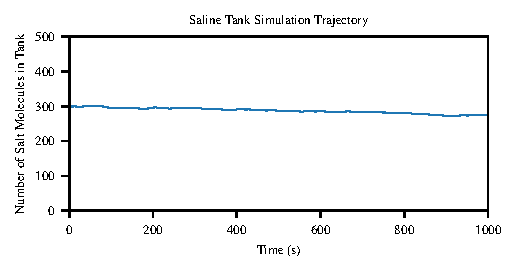
\includegraphics[width=\textwidth]{figures/saline_tank.pdf}
\caption{An example simulation from the model of Example~\ref{ex:saline_tank} with initial
condition $M(0) = 300 \textup{ NaCl molecules}$, parameters $V = 10^6\textup{ liters}$,
$a = b = 100\textup{ liters per hour}$,
$c=2.9112 \times 10^{-26}\textup{ grams per liter}$, assuming that one NaCl molecule has
mass $m = 9.704 \times 10^{-23}\textup{ grams}$, and with runtime $T=10^3\textup{ hours}$. We draw this with \PlotTrajs{} from \texttt{tools/plots/plot\_trajectories.py} (Listing~\ref{lst:plots_trajectories}).}
\label{fig:saline_tank}
\end{figure}

\end{example}


\begin{example}\label{ex:logistic_growth_code}
\textbf{Logistic Growth DG Simulation.}
Reconsider Example~\ref{ex:logistic_growth}, the logistic growth model. It is the simplest of our models: the state $P$ is a single population count changed by exactly two events. A birth increases $P$ by one and occurs at rate $rP$, and a death decreases $P$ by one and occurs at rate $rP^2/K$, where $r$ is the per-capita birth rate and $K$ is the carrying capacity. Table~\ref{tab:ode_events} lists the two events.

We simulate with a base doubling time $\tau = 36.5$ days, so that $r = \ln(2)/\tau$, a carrying capacity $K = 200$, an initial population $P(0) = 20$, and a run time $T = 365$ days.

In Figure~\ref{fig:bespoke_logistic_growth}, $\textsf{MakeRates}$ returns the birth rate $rP$ and the death rate $rP^2/K$ of Table~\ref{tab:ode_events}, and $\textsf{MakeDeltaStates}$ returns the state-change vector $(+1, -1)$, the $+1$ for a birth and the $-1$ for a death. Listing~\ref{lst:framework_logistic_growth} gives the \texttt{Python} implementation. It diverges from the pseudocode in deriving the per-capita rate $r = \ln(2)/\tau$ from the base doubling time, rather than taking $r$ directly.

\begin{figure}[htbp]
\centering
{\footnotesize
\adjustbox{valign=t}{\fbox{\procedure{$\textsf{MakeRates}(P,\, \theta) \to \vec{\lambda}$:}{
\pcind \pcreturn \left(rP,\; rP^2/K\right)
}}}\qquad
\adjustbox{valign=t}{\fbox{\procedure{$\textsf{MakeDeltaStates}(\theta) \to (\delta_j)_{j=1}^{N}$:}{
\pcind \pcreturn (+1,\, -1)
}}}\par}
\caption{The two bespoke subroutines for the logistic growth model. $\textsf{MakeRates}$ returns the birth and death rates, and $\textsf{MakeDeltaStates}$ returns the $\pm 1$ state changes, both following Table~\ref{tab:ode_events}. Compare to the \texttt{Python} in Listing~\ref{lst:framework_logistic_growth}.}
\label{fig:bespoke_logistic_growth}
\end{figure}

\lstinputlisting[float=htbp, language=Python, numbers=none, linerange={29-37}, caption={The bespoke \texttt{Python} functions for the logistic growth model, \MakeLogisticRates{} and \MakeLogisticDeltaStates{}. We pair these with the pseudocode of Figure~\ref{fig:bespoke_logistic_growth}.}, label={lst:framework_logistic_growth}]{../simulation_frameworks/logistic_growth.py}

The stochastic trajectories fluctuate around the deterministic logistic solution. Figure~\ref{fig:logistic_growth_mean_vs_ode} compares the mean of $30$ stochastic trajectories against the solution of Equation~\ref{eqn:logistic_growth}.

\end{example}


\begin{example}\label{ex:allee_code}
\textbf{Allee Effect DG Simulation.}
Reconsider Example~\ref{ex:allee} and the emperor's goal to estimate the probability that a colony goes extinct. We simulate trajectories with run times $T=2000$ days each and compute the sample proportion of simulations that go extinct. We assume the species has a base birth rate\index{birth rate} $r = 0.0045\textup{ days}^{-1}$, a cooperation threshold $L = 50\textup{ individuals}$, and a carrying capacity\index{carrying capacity} $K = 200\textup{ individuals}$. All colonies begin with $P(0) = 50$ individuals.

This system with these parameters has three equilibria. $P = 0$ and $P = K$ are stable equilibria, and $P = L$ is an unstable equilibrium. Trajectories with $0 < P < L$ or $P > K$ drift downward statistically. Trajectories with $L < P < K$ drift upward statistically. Since simulations start with $P(0) = 50 = L$, the first event is equally likely to be a birth or a death. About half of all trajectories will initially decrease and drift toward extinction. We therefore expect about half of all trajectories to end in extinction. Extinction is a permanent condition. Table~\ref{tab:allee_events} lists the four events.

\begin{table}[htbp]
\centering
\caption{Allee effect Doob-Gillespie events.}\label{tab:allee_events}
\begin{tabular}{llll}
\hline
Event & Description & Rate & $\Delta$State \\
\hline
Old-age death & Individual dies of old age & $\lambda_0 P$ & $-1$ \\
Sexual birth & Birth from sexual reproduction & $\lambda_0 P^2/K$ & $+1$ \\
Cooperative birth & Birth from cooperation & $\lambda_0 P^2/L$ & $+1$ \\
Competitive death & Death from over-competition & $\lambda_0 P^3/(KL)$ & $-1$ \\
\hline
\end{tabular}
\end{table}

In Figure~\ref{fig:bespoke_allee}, $\textsf{MakeRates}$ returns the four rates of Table~\ref{tab:allee_events} as the vector $(rP,\, rP^2/K,\, rP^2/L,\, rP^3/(KL))$, and $\textsf{MakeDeltaStates}$ returns the state-change vector $(-1, +1, +1, -1)$. Listing~\ref{lst:framework_allee} gives the \texttt{Python} implementation.

\begin{figure}[htbp]
\centering
{\footnotesize
\adjustbox{valign=t}{\fbox{\procedure{$\textsf{MakeRates}(P,\, \theta) \to \vec{\lambda}$:}{
\pcind \pcreturn \left(rP,\; \frac{r P^2}{K},\; \frac{r P^2}{L},\; \frac{r P^3}{KL}\right)
}}}\qquad
\adjustbox{valign=t}{\fbox{\procedure{$\textsf{MakeDeltaStates}(\theta) \to (\delta_j)_{j=1}^{N}$:}{
\pcind \pcreturn (-1,\, +1,\, +1,\, -1)
}}}\par}
\caption{The two bespoke subroutines for the Allee effect model, following Table~\ref{tab:allee_events}. Here $r$ is the base per-capita birth rate. Compare to the \texttt{Python} in Listing~\ref{lst:framework_allee}.}
\label{fig:bespoke_allee}
\end{figure}

The function \FindTraj{} (in the Python repository) inputs simulation setup data and a success condition function and returns a successful trajectory with a count of all attempts including the successful one. After running the Allee effect script (in the Python repository) with a sample of $128$ simulations, we saw $71$ simulations go extinct, providing an estimated probability of extinction $\widehat{p} = 0.5546875$ (see Section~\ref{subsec:background} for the definition of sample proportion and hat notation).
Verify that the qualitative behavior matches your ODE analysis: trajectories starting below $P = L = 50$ should drift toward extinction, while those starting above $L$ should drift toward $K = 200$.

\lstinputlisting[float=htbp, language=Python, numbers=none, linerange={9-19}, caption={\texttt{Python} functions \MakeAlleeRates{} and \MakeAlleeDeltaStates{} for the Allee effect model. See pseudocode in Figure~\ref{fig:bespoke_allee}.}, label={lst:framework_allee}]{../simulation_frameworks/allee_effect.py}

\begin{figure}[htbp]
\centering
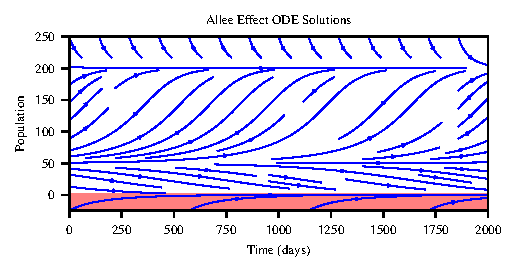
\includegraphics[width=\textwidth]{figures/allee_ode.pdf}
\caption{Phase diagram for Allee effect ODE $\frac{dP}{dt} = -rP(1-P/L)(1-P/K)$ ()$r = 0.0045\,\text{days}^{-1}$, $L = 50$, $K = 200$, from Example~\ref{ex:allee}).
Trajectories below $P = L$ trend to extinction. Trajectories above $P = L$ trend to $P = K$.
We shade the non-physical region $P < 0$ red. We draw this with \MakePhaseDiagram{} from \texttt{tools/plots/plot\_vector\_field.py} (Listing~\ref{lst:plots_vector_field}).}
\label{fig:allee_ode}
\end{figure}

\begin{figure}[htbp]
\centering
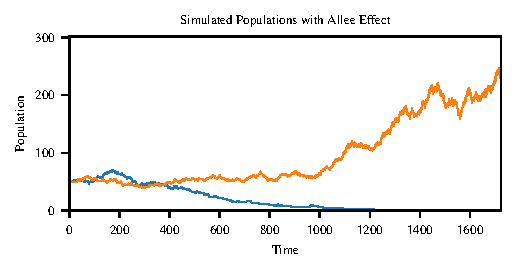
\includegraphics[width=\textwidth]{figures/allee_effect_two_trajs.pdf}
\caption{Two Allee trajectories from
Example~\ref{ex:allee}, with $r = 0.0045 (\text{time})^{-1}$,
$L = 50 \text{individuals}$, $K = 200$, and  $P(0) = 50$.  We draw this with \PlotTrajs{} from \texttt{tools/plots/plot\_trajectories.py} (Listing~\ref{lst:plots_trajectories}).}
\label{fig:allee_two_trajs}
\end{figure}


\begin{figure}[htbp]
\centering
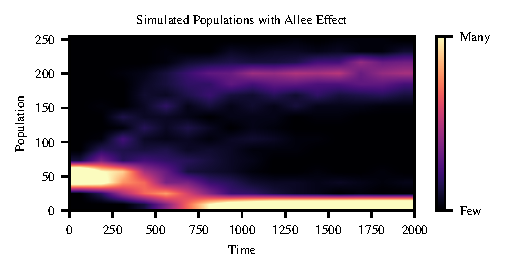
\includegraphics[width=\textwidth]{figures/allee_effect.pdf}
\caption{Heat map of $128$ Allee trajectories from Example~\ref{ex:allee} with the same parameters as Figure \ref{fig:allee_two_trajs}. Brighter pixels are near more trajectories.
We draw this with \PlotHeatmap{} from \texttt{tools/plots/plot\_heatmap\_histogram.py} (Listing~\ref{lst:plots_heatmap}).}
\label{fig:allee_heat}
\end{figure}

There are two types of stochastic trajectory. \textit{Successful} trajectories drift above $P(t) = L$ and reach the carrying capacity $P(t) = K$. \textit{Unsuccessful} trajectories slip below $P(t) = L$ and decline to extinction.
We use \PlotExtinctionAndSurvival{} to find two such trajectories in Figure~\ref{fig:allee_two_trajs}. See Section~\ref{subsec:plotting_utilities} for the plotting code.
The underlying ODE is scalar. We can therefore draw its phase diagram (Figure~\ref{fig:allee_ode}) as a streamplot in the $(t, P)$ plane. The streamlines confirm the three equilibria $P \in \{0, L, K\}$: trajectories starting below $L = 50$ converge to extinction, while those starting between $L$ and $K$ converge to the carrying capacity.
We generate a heat map of $128$ stochastic trajectories of the Allee model in Figure~\ref{fig:allee_heat}.
Nearly all trajectories fall into one of these two categories.
The heat map in Figure~\ref{fig:allee_heat} shows a proportion of simulations sweeping upward to the stable carrying capacity $P=K=200$, as well as a proportion falling below $P=L=50$ and ending near or at extinction.
The bright horizontal band around $P = 0$ at the end of the simulation indicates that many trajectories end in extinction.
The horizontal smear of brightness around $P = K = 200$ at the end of the simulation indicates that some trajectories survive at carrying capacity.
The darkness everywhere else indicate that trajectories don't spend a lot of time in the intermediate regions.
Hence, the distribution of simulation results at the end of the simulation is bimodal,\index{distribution!bimodal} with a cluster around $P = 0$ and a cluster around $P = K$.

As an aside, the state $P = 0$ is an absorbing state, so every window containing $P = 0$ contains many trajectories by the end of the simulation.
Thus, $P = 0$ appears very bright. In fact, in our Python code, we had to cap brightness to ensure that multimodal distributions would be visible.
The state $P = K$ is only probabilistically attracting, showing brightness in a haze around it, but trajectories wander nearby, dissipating their heat.
To make this graph, the heat map routine resamples every trajectory onto a common uniform time grid and then performs simple histogram binning.
That is to say, the heat indicates the residence of nearby trajectories, not the absolute number of nearby change-points.
See Section~\ref{subsec:plotting_utilities} for the heat-map plotting code and Section~\ref{subsubsec:prep_heatmap} for an explanation of this resampling.



The simulations are stochastic. Exceptions occur occasionally: trajectories bound for extinction that randomly wander above $P=L$ and recover to $P=K$, or trajectories near $P=K$ that randomly wander below $P=L$.

\end{example}


\begin{example}\label{ex:sir_code}
\textbf{SIR DG Simulation.}
Reconsider Example~\ref{ex:sir_first} and Charlie's fungus-infected cats. The SIR model partitions a population into three compartments: susceptible ($S$), infectious ($I$), and recovered ($R$). Individuals move from $S$ to $I$ upon infection and from $I$ to $R$ upon recovery. Assume Charlie has $S + I + R = 100$ cats, assume $I(0) = 10$ of the cats start out sick, and assume the rest are susceptible. We assume that cats recover with a half-life $\tau = 45$ days and interact with each other in random pairs $1000$ times a day, so the time between a cat's interactions is $\tau_{\textup{int}} = 1/1000 = 0.001$ days, and each interaction has a probability $0.0001$ (that is, $0.01\%$) of an infection spreading.
We use $\widetilde{\alpha} = \frac{0.0001}{0.001} = 0.1\,\textup{days}^{-1}$, and since $S + I + R = N = 100$, the per-pair rate is $\alpha = \widetilde{\alpha}/N = \frac{0.0001}{0.001 \cdot 100} = 10^{-3}\,(\textup{individual}\cdot\textup{days})^{-1}$, matching \MakeSirRates{} in the companion code.

We re-parameterize in terms of daily interactions because transmissibility depends on both the infectious organism and social behavior. For example, the black-tailed prairie dog is sociable, and plague (\textit{Yersinia pestis}) infections transmit rapidly through their populations. By contrast, California ground squirrels (\textit{Otospermophilus beecheyi}) are less social in their burrowing behavior and tolerate plague better than black-tailed prairie dogs \cite{buhnerkempe2011transmission}.

Unlike the previous models, the SIR state is a vector $(S, I, R)$ rather than a scalar count. Table~\ref{tab:sir_dg_events} lists the two events and their vector state changes.

\begin{table}[htbp]
\centering
\caption{SIR Doob-Gillespie events.}\label{tab:sir_dg_events}
\begin{tabular}{llll}
\hline
Event & Description & Rate & $\Delta$State \\
\hline
Infection & Susceptible becomes infectious & $\alpha S I$ & $(-1,+1,0)$ \\
Recovery & Infectious individual recovers & $\beta I$ & $(0,-1,+1)$ \\
\hline
\end{tabular}
\end{table}

In Figure~\ref{fig:bespoke_sir}, $\textsf{MakeRates}$ returns the infection rate $\alpha S I$ and the recovery rate $\beta I$ of Table~\ref{tab:sir_dg_events}, and, because the state is the vector $(S, I, R)$, $\textsf{MakeDeltaStates}$ returns the two vector changes $(-1, +1, 0)$ for an infection and $(0, -1, +1)$ for a recovery. Listing~\ref{lst:framework_sir} gives the \texttt{Python} implementation. It diverges from the pseudocode in two language- and model-specific ways: it derives $\alpha$ from the interaction time and infection probability and $\beta = \ln(2)/\tau$ from the recovery half-life, rather than taking $\alpha$ and $\beta$ directly, and it adds the chosen state change componentwise in \UpdateSirState{}.

\begin{figure}[htbp]
\centering
{\footnotesize
\adjustbox{valign=t}{\fbox{\procedure{$\textsf{MakeRates}((S,I,R),\, \theta) \to \vec{\lambda}$:}{
\pcind \pcreturn \left(\alpha S I,\; \beta I\right)
}}}\qquad
\adjustbox{valign=t}{\fbox{\procedure{$\textsf{MakeDeltaStates}(\theta) \to (\delta_j)_{j=1}^{N}$:}{
\pcind \pcreturn \left((-1, +1, 0),\; (0, -1, +1)\right)
}}}\par}
\caption{The two bespoke subroutines for the SIR model, following Table~\ref{tab:sir_dg_events}. Here $\alpha$ is the transmission rate and $\beta$ the recovery rate. The state change $\delta_j$ is a vector. Compare to the \texttt{Python} in Listing~\ref{lst:framework_sir}.}
\label{fig:bespoke_sir}
\end{figure}

\lstinputlisting[float=htbp, language=Python, numbers=none, linerange={13-29}, caption={The bespoke \texttt{Python} functions for the SIR model: \MakeSirRates{}, \MakeSirDeltaStates{}, and the componentwise update \UpdateSirState{}. We pair these with the pseudocode of Figure~\ref{fig:bespoke_sir}.}, label={lst:framework_sir}]{../simulation_frameworks/epidemiology.py}

We generate $100,000$ stochastic trajectories with run time $T = 365$ days (see the Python repository for the code) to estimate (i) the probability that Charlie's cats totally recover within a year and (ii) the five-number summary\index{summary, five-number} of the time until Charlie has no more infected cats, computed from trajectories in which all infectious cats recovered (i.e., $I = 0$) before day $365$. Our simulation reveals an estimated probability of total recovery within the year of $0.53844$ (a sample proportion, defined in Section~\ref{subsec:background}). The five-number summary (see Section~\ref{subsec:background}) of the time until recovery, computed only from trajectories in which all infectious cats recovered before day $365$, was $(161.5, 288.1, 315.9, 340.0, 364.998)$. This indicates that, when Charlie's cats totally recover within one year, a $50\%$ probability exists that the cats will take more than $316$ days to recover. We use the SIR plotting code (in the Python repository) to visualize one representative stochastic trajectory (which includes all three compartments of population members) in Figure~\ref{fig:sir}.

\begin{figure}[htbp]
\centering
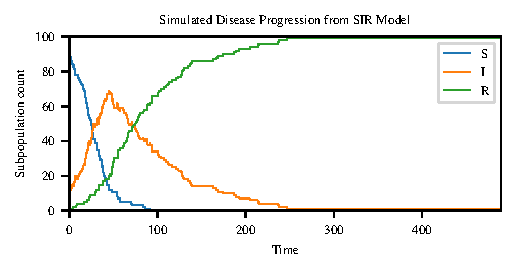
\includegraphics[width=\textwidth]{figures/epidemiology.pdf}
\caption{An example simulation of the fungal infection among Charlie's cats, showing the susceptible ($S$), infectious ($I$), and recovered ($R$) compartments over time. We draw this with \PlotTrajs{} from \texttt{tools/plots/plot\_trajectories.py} (Listing~\ref{lst:plots_trajectories}).}
\label{fig:sir}
\end{figure}

Verify that the qualitative behavior matches your ODE analysis: the susceptible compartment should fall monotonically, and the infectious compartment should peak and then decline as recovery outpaces new infections.

A streamplot like Figure~\ref{fig:ode_examples} does not apply here. A streamplot in the $(t, x)$ plane depicts the vector field $(1, f(t,x))$ for a scalar ODE $\dot{x} = f(t,x)$. The SIR state is the vector $(S, I, R)$ with conservation law $S + I + R = N$. The individual rates $\frac{dS}{dt} = -\alpha SI$ and $\frac{dI}{dt} = \alpha SI - \beta I$ each depend on two compartments. A phase portrait in the $(S, I)$ plane is possible, but it discards the time axis and does not give the timescale of the outbreak.

\end{example}




The examples above used sample proportions and five-number summaries to summarize simulation output. Section~\ref{subsec:background} introduces both. Section~\ref{subsec:output} formalizes their use, discusses when summary statistics can be misleading (particularly for bimodal output), and provides practical guidance for reporting stochastic simulation results. Read Section~\ref{subsec:output} before proceeding to sensitivity analysis (Section~\ref{subsec:qualitative_changes}), as the sensitivity analysis in Section~\ref{subsec:qualitative_changes} relies on the same statistical vocabulary.

\textup{{\bf Questions for Reflection:}}
\begin{enumerate}

\item Given $r, s > 0$ and the same initial condition $X_0 = Y_0$, the ODEs $\frac{dX}{dt} = rX$ and $\frac{dY}{dt} = (r+s)Y - sY$ always produce the same trajectories. Can you use the Doob-Gillespie algorithm to detect a difference between them? Explain.

\item In the deterministic Allee ODE, what happens as $L$ approaches $K$?

\item What can we expect from stochastic realizations of the Allee ODE as $L$ approaches $K$?

\item In the deterministic Allee ODE, what happens as we vary $r$?

\item What are some changes we can expect from the stochastic realizations of the Allee ODE as we vary $r$?

\item Consider the Allee-like model $\frac{dY}{dt} = rY(1-\frac{Y}{K})(1-\frac{Y}{L})(1-\frac{Y}{U})$ for some $K > L > U > 0$. Is this model suitable for describing a realistic ecological population with finite resources? Hint: Find the equilibria and determine whether birth or death is more likely near those equilibria.

\item How does your answer to the previous question change if we use $\frac{dY}{dt} = -rY(1-\frac{Y}{K})(1-\frac{Y}{L})(1-\frac{Y}{U})$ with the same $K > L > U > 0$? Hint: The sign change reverses time.

\item Interpret the notion of stochastic extinction with respect to the SIR model as presented in Example~\ref{ex:sir_first} as the occurrence that $S$ or $I$ randomly crashes to zero, and explain the impact on the remainder of the simulation when either of these compartments crashes to zero.

\item If an ODE has no oscillations near an equilibrium, the trajectories produced by the Doob-Gillespie algorithm are still stochastic and go up and down randomly, giving the illusion of oscillation. On the other hand, even if an ODE has oscillations near an equilibrium, the Doob-Gillespie trajectories are stochastic and may be strictly increasing or strictly decreasing for long intervals of time. Think about ways to detect whether a stochastic Doob-Gillespie implementation comes from an ODE that has oscillations.

\item After no susceptibles remain in the SIR model, $I$ changes like in the radioactive decay model with rate of decay $\beta$. Using $\beta = \ln(2)/45 \approx 0.0154\text{ days}^{-1}$, compute the ``half-life'' and interpret this half-life in terms of the original phenomena described by the SIR model. Check whether your computation of half-life makes sense by comparing it with Figure~\ref{fig:sir}.


\end{enumerate}

\section{Visualizing and Interpreting Simulated Trajectories}\label{sec:visualizing_interpreting}

%\textbf{Instructional Time:} 3 hours

\subsection{Visualizing Simulated Trajectories}\label{subsec:visualizing}

Section~\ref{sec:farming} produces trajectories. This subsection addresses how to display them. We plot stochastic trajectories rather than phase diagrams of deterministic ODE solutions. These trajectories hover near the deterministic solution but are noisy, discrete-state realizations, not smooth curves.

\subsubsection{A single trajectory is a step function}\label{subsubsec:single_traj_step}

Because the DG algorithm changes the state by exactly one integer at each event, the state remains constant between events and jumps discontinuously at each one. Thus, a stochastic trajectory the DG algorithm simulates is a piecewise-constant function\index{function!piecewise-constant} of time: the state holds constant between consecutive change points\index{change point} and jumps by $\pm 1$ at each event.

Consider a single run of the saline tank model (Example~\ref{ex:saline_tank_code}). The state variable is $M$, the number of NaCl molecules. The tank starts at $M = 300$ NaCl molecules. The deterministic equilibrium is $M \approx 150$, so the system is initially above equilibrium: departures are more likely than arrivals. After an exponentially distributed waiting time, the first event occurs. Suppose it is a departure. The state steps down to $M = 299$. We sample a new waiting time, the second event occurs, and the state steps again. The process repeats. Wait-times are random, so the events do not spread evenly in time. Sometimes, events occur often, with very little wait time. Sometimes, events occur seldomly, with long periods of stagnation. Over simulated time, many such steps accumulate. The result is a noisy staircase that drifts downward toward equilibrium and then fluctuates around it indefinitely.

This staircase is the raw output of the DG algorithm. Each changepoint $(t_i, M_i)$ is a corner of the step function, and the state is constant on each time interval $[t_i, t_{i+1})$. See Section~\ref{subsec:plotting_utilities} for the code that renders a stochastic trajectory as a step graph.

\subsubsection{Every run is different: motivating the heat map}\label{subsubsec:motivating_heatmap}

One trajectory is one sample from a distribution. Just as a single coin flip does not reveal the bias of the coin, a single trajectory does not reveal the probability of extinction or the range of typical outcomes.

Each run of the DG algorithm yields a distinct staircase. Two runs with the same initial conditions and parameters will agree in trend but differ in every individual step, because each waiting time and each event choice is random. Running the simulation $100{,}000$ times produces $100{,}000$ different staircases (usually).

If every run is different, how do we summarize all of them?

One approach is to overlay all trajectories on a single plot. For a small number of trajectories this works well, as seen in Figure~\ref{fig:allee_two_trajs}. For thousands of trajectories it produces an unreadable smear.

A more informative approach is a heat map:\index{heat map} a two-dimensional histogram over the $(t, Y)$-plane in which the color intensity of each cell is proportional to the number of simulated trajectories that pass through that cell. Cells that many trajectories visit appear bright. Cells that few visit appear dark. The heat map renders $100{,}000$ step functions as a single image. It shows whether the distribution of the state at a given time is unimodal,\index{distribution!unimodal} bimodal,\index{distribution!bimodal} or multimodal.

\subsubsection{Preparing trajectories for a heat map}\label{subsubsec:prep_heatmap}

Bright regions in a heat map show where many trajectories spend time. Multiple bright spots signal bimodal behavior.

The DG algorithm outputs change points at random times, not on a regular grid. To aggregate trajectories into a grid-based heat map, the heat map routine resamples every trajectory onto a common, uniform time grid before binning.
This piecewise-constant interpolation records the state at each grid time using the most recent changepoint, converting a sparse list of change points into a dense list of $(t, Y)$ pairs suitable for binning.

Filling at a random or too-coarse spacing introduces a small bias\index{heat map!binning bias} into the heat map.
When events occur frequently relative to the grid, several change points can fall between consecutive grid points, so the grid samples miss them and over-represent the states that happen to lie on grid lines. The bias worsens as events become more frequent. A finer partition reduces it, and we can show the error is $O(\Delta)$ in the grid spacing $\Delta$.
However, as $\Delta \to 0$, the graph approaches the unreadable smear we get when plotting all trajectories plainly, and there's a trade-off in cost. A heatmap with grid spacing $\Delta$ requires painting $O(\Delta^{-2})$ pixels. So in practice, we hand-tune $\Delta$ to get an informative heat map.

See Section~\ref{subsec:plotting_utilities} for the heat-map plotting code.

\subsection{The Plotting Utilities}\label{subsec:plotting_utilities}

We draw every figure in this chapter with one of four single-function modules in \texttt{tools/plots/}.
These modules are plotting code, not algorithms, so they have no pseudocode counterpart.
The scripts in \texttt{scripts/} use these tools to make the figures.
This way, the scripts play double duty as usage examples.

Three of our plotting utilities share one structure, the template of Listing~\ref{lst:plots_template}: set the page style, draw, then save or show.
Recall the template in Figure~\ref{fig:dg_algorithm} and Listing~\ref{lst:dg_algorithm_python_template} uses $\texttt{...}$ to mark the block in the DG algorithm which we must tailor for the ODE model.
Similarly, we use \texttt{...} to mark the block in the plotting template which we must tailor for the kind of image we generate.
The heat map follows the same template, but with an additional block that prepares the trajectories for binning before drawing.

Our plotting template's styling preamble converts two width fractions into \texttt{matplotlib} settings.
Publishers often resize images in LaTeX. The fraction \texttt{width\_frac} is the figure width as a fraction of the text width and \texttt{display\_frac} is the fraction at which we place the figure on the page, so their ratio \texttt{scale} undoes any later shrinkage.
The size \texttt{on\_page\_pt} is one point below the $10$-point body, which we rescale by \texttt{scale} to ensure that graph titles, legends, and labels have a common font size with the body. We store the width of the figure in inches in \texttt{width}.
Python's dictionary comprehension is sort of like set builder notation. We use it to store \texttt{on\_page\_pt} as font sizes for titles, labels, and legends in the dictionary \texttt{rc}. We use \texttt{rc.update} to add the serif font family, the STIX math font, $150$ dpi, the figure size, and a scaled line width. When a \texttt{latex} executable is on the path, the code enables \texttt{usetex} to match fonts. Writing \texttt{rc} into \texttt{rcParams} applies the settings.

After the drawing block, the tail sets the title and axis labels, tightens the margins, and either writes the figure to \texttt{save\_path}, creating its directory first, or shows it on screen.

\lstinputlisting[float=htbp, language=Python, numbers=none, caption={The shared template for the \texttt{tools/plots/} plotters. The styling preamble and the save-or-show tail are common to the trajectory, phase-diagram, and mean-versus-ODE plotters; each replaces the \texttt{...} block with its own drawing.}, label={lst:plots_template}]{../tools/plots/plot_template.py}

\subsubsection{Plotting trajectories}\label{subsubsec:code_plot_trajs}

The drawing block of \PlotTrajs{} (Listing~\ref{lst:plots_trajectories}) renders trajectories as step graphs. \texttt{draw\_labels} substitutes a list of \texttt{None} when the caller gives no labels, keeping the loop uniform. The loop unzips each trajectory into times and states and draws it as a right-continuous step (\texttt{where='post'}). A legend appears only when the caller supplies real labels. The \texttt{xlim} and \texttt{ylim} calls fix the axis ranges to the supplied bounds.

\lstinputlisting[float=htbp, language=Python, numbers=none, linerange={29-37}, caption={The drawing block of \PlotTrajs{} in \texttt{tools/plots/plot\_trajectories.py}, which we insert into the template of Listing~\ref{lst:plots_template}. It draws Figures~\ref{fig:saline_tank}, \ref{fig:allee_two_trajs}, and~\ref{fig:sir}.}, label={lst:plots_trajectories}]{../tools/plots/plot_trajectories.py}

\subsubsection{Plotting phase diagrams}\label{subsubsec:code_phase}

The drawing block of \MakePhaseDiagram{} (Listing~\ref{lst:plots_vector_field}) draws the streamplot of a scalar ODE. \texttt{mgrid} builds a grid of resolution \texttt{res} over the time-state rectangle. The horizontal arrow component is $1$ since time advances at unit rate, and the vertical component is the caller's \texttt{y\_len\_fun} on the grid. To use this to make a phase diagram of an ODE of the form $y^\prime = f(y)$, just express $f(y)$ as \texttt{y\_len\_fun}. The \texttt{streamplot} call draws the field in blue with arrow size scaled to the page, and an optional \texttt{axhspan} shades the non-physical region below zero red.

\lstinputlisting[float=htbp, language=Python, numbers=none, linerange={31-38}, caption={The drawing block of \MakePhaseDiagram{} in \texttt{tools/plots/plot\_vector\_field.py}, which we insert into the template of Listing~\ref{lst:plots_template}. It draws the phase diagrams in Figures~\ref{fig:ode_examples} and~\ref{fig:allee_ode}.}, label={lst:plots_vector_field}]{../tools/plots/plot_vector_field.py}

\subsubsection{Plotting the mean against the ODE}\label{subsubsec:code_mean}

The drawing block of \PlotMeanVsOde{} (Listing~\ref{lst:plots_mean_vs_ode}) overlays a stochastic mean on a deterministic solution. An optional \texttt{axhspan} shades the non-physical region. The code plots the stochastic mean as a solid curve and the ODE solution as a dashed curve, sets the axes to the data range, and places a legend at the lower right.

\lstinputlisting[float=htbp, language=Python, numbers=none, linerange={29-35}, caption={The drawing block of \PlotMeanVsOde{} in \texttt{tools/plots/plot\_mean\_vs\_ode.py}, which we insert into the template of Listing~\ref{lst:plots_template}. It draws Figure~\ref{fig:logistic_growth_mean_vs_ode}.}, label={lst:plots_mean_vs_ode}]{../tools/plots/plot_mean_vs_ode.py}

\subsubsection{Plotting the heat map}\label{subsubsec:code_heatmap}

The heat map follows the template, adding a block that prepares the trajectories before the drawing block.
\PlotHeatmap{} (Listing~\ref{lst:plots_heatmap}) first re-samples trajectories by laying \texttt{grid} equal time bins, finding their centers, and reading each trajectory's state at those centers by looking at the latest change point with \texttt{searchsorted}. Section~\ref{subsubsec:prep_heatmap} explains why this matters. \PlotHeatmap{} then stacks the re-sampled trajectories. \texttt{histogram2d} bins the $(t, y)$ pairs into a \texttt{grid}-by-\texttt{grid} count array. This count array determines brightness, but we cap the brightness at the $95$th percentile of counts as \texttt{vmax}. This way, the brightest cells saturate while dimmer occupancy bands stay visible, showing multimodal distributions. Finally, the code draws the transposed counts as a rasterized image with the \texttt{magma} colormap and bilinear smoothing, adds a color bar labeled from \emph{Few} to \emph{Many}, labels the axes, and saves or shows the figure through the shared tail.

\lstinputlisting[float=htbp, language=Python, numbers=none, linerange={30-55}, caption={The drawing block of \PlotHeatmap{} in \texttt{tools/plots/plot\_heatmap\_histogram.py}, which we insert into the template of Listing~\ref{lst:plots_template}. It draws the heat map in Figure~\ref{fig:allee_heat}.}, label={lst:plots_heatmap}]{../tools/plots/plot_heatmap_histogram.py}

\subsection{Reading and Statistically Measuring Stochastic Output}\label{subsec:output}

%\textbf{Instructional Time:} 1 hour

Examples~\ref{ex:saline_tank_code}, \ref{ex:allee_code}, and \ref{ex:sir_code} reported results as sample proportions and five-number summaries without justifying why these statistics are appropriate or how to interpret them. We provide a light refresher on statistics in this section.

\subsubsection{Sample proportion as a probability estimator}\label{subsubsec:sample_proportion}

As a rule, if the event has probability $p$, run at least $1/p$ simulations to observe it reliably. For rare events ($p$ near $0$), you need much larger samples.

Many questions about a model reduce to a binary outcome: does the population go extinct? Does the process succeed before time $T$? Does the state ever exceed a threshold? For any such binary event with true probability $p$, a large sample of $n$ independent simulations, and $k$ observations, the sample proportion\index{proportion, sample} $\hat{p} = k/n$ is an unbiased estimator\index{estimator, unbiased} of $p$: on average, $\hat{p} = p$. The precision of $\hat{p}$ improves as $n$ increases, with standard error $\sqrt{p(1-p)/n}$.

If $\hat{p} = 3/100{,}000 = 3\times 10^{-5}$, the estimate is not robust: observing even one less observation would reduce our estimate to $2/100{,}000$, a $50\%$ drop.

\subsubsection{Five-number summary for a continuous-valued statistic}\label{subsubsec:five_number}

The mean is misleading for skewed or multimodal distributions. The five-number summary\index{summary, five-number} describes center, spread, and extremes without assuming a symmetric shape.

When the statistic of interest is continuously valued (for example, the time until extinction, the time until full recovery, or the peak state), the five-number summary (see Section~\ref{subsec:background}) provides a concise description of the distribution without assuming any parametric form.

In Example~\ref{ex:sir_code}, we restricted to the simulations in which all cats recovered within the year.
We computed the five-number summary of the recovery time and saw the following.
\begin{itemize}
\item The fastest recovery took about $161.5$ days ($Q_0 = \min$).
\item The median recovery time was about $316$ days.
\item $75\%$ of recoveries took more than $288$ days ($Q_1$).
\item The slowest recovery in the sample reached $364.998$ days ($Q_4 = \max$), strictly inside the simulation window.
\end{itemize}
Determining these statistics requires no distributional assumption (normal, exponential, etc.). We call the five-number summary \textit{non-parametric}.

\subsubsection{Non-unimodal distributions and their interpretation}\label{subsubsec:non_unimodal}

Before coming to any conclusions, inspect whether the distribution is unimodal. Conclusions based on the mean or median for a strongly bimodal or multimodal distribution is misleading, because the central value may fall in a trough between two peaks where few trajectories reside.

The Allee effect simulation (Example~\ref{ex:allee_code}) illustrates this. The heat map in Figure~\ref{fig:allee_heat} shows two distinct clusters of trajectories at the end of the simulation: one near the stable carrying capacity $K = 200$ and one near extinction\index{extinction!stochastic} at $P = 0$. The distribution of final states is strongly bimodal. A single average final state conveys almost no useful information.

The conditional distribution of the final state given survival, i.e.\ the \textit{survivorship bias}, is more informative, but is misleading for its own reasons. Statistical patterns which matter only indirectly are less informative than direct causes, and those are less informative than firm predictions. Like a good prediction of weather should provid a probability of rain, a good analysis of a population ecology model should estimate extinction probability $\hat{p}$.

No matter the stastics we decide to measure, it is wise to inspect a heat map or histogram of the simulation output. If the distribution has more than one mode, partition the trajectories into qualitatively distinct groups and perform separate statistical analyses for each group.

\textup{{\bf Questions for Reflection:}}
\begin{enumerate}
\item A social researcher finds that the average American family has decreased in size from $1.7$ parents and $2.3$ children to $1.1$ parents and $1.9$ children. Explain why this might be misleading and discuss what you would report instead.

\item The heat map of the Allee effect simulation shows two bright bands at $P = 0$ and $P = K$ at time $T$; extinction appears highly likely, say with probability $p$. Using the standard-error rule from Section~\ref{subsec:output}, approximately how many simulations do you need to estimate $p$ with a standard error of at most $0.01$?

\item The heat map routine records the state at each grid time using the last observed state before that time. A colleague suggests linear interpolation between change points instead. Describe one scenario in which linear interpolation would give a visually smoother heat map yet misrepresent the true probability distribution of the process.
\end{enumerate}

